\section{Notes on the proposed tactics and topics for the related work chapter}~\label{rw-proposed-tactics-and-topics-for-this-chapter}

Where others have done similar work they've done so in other ways eg MSR rather than focusing on the development teams. When I observed the teams the effects of the processes, artefacts, and the tools emerged. This is why I've picked these 3 aspects and 6 perspectives. 

\subsection{Some notes on the methods used for the literature review}~\label{rw-notes-on-methods-used-for-literature-review-topic}

\begin{figure}
    \centering
    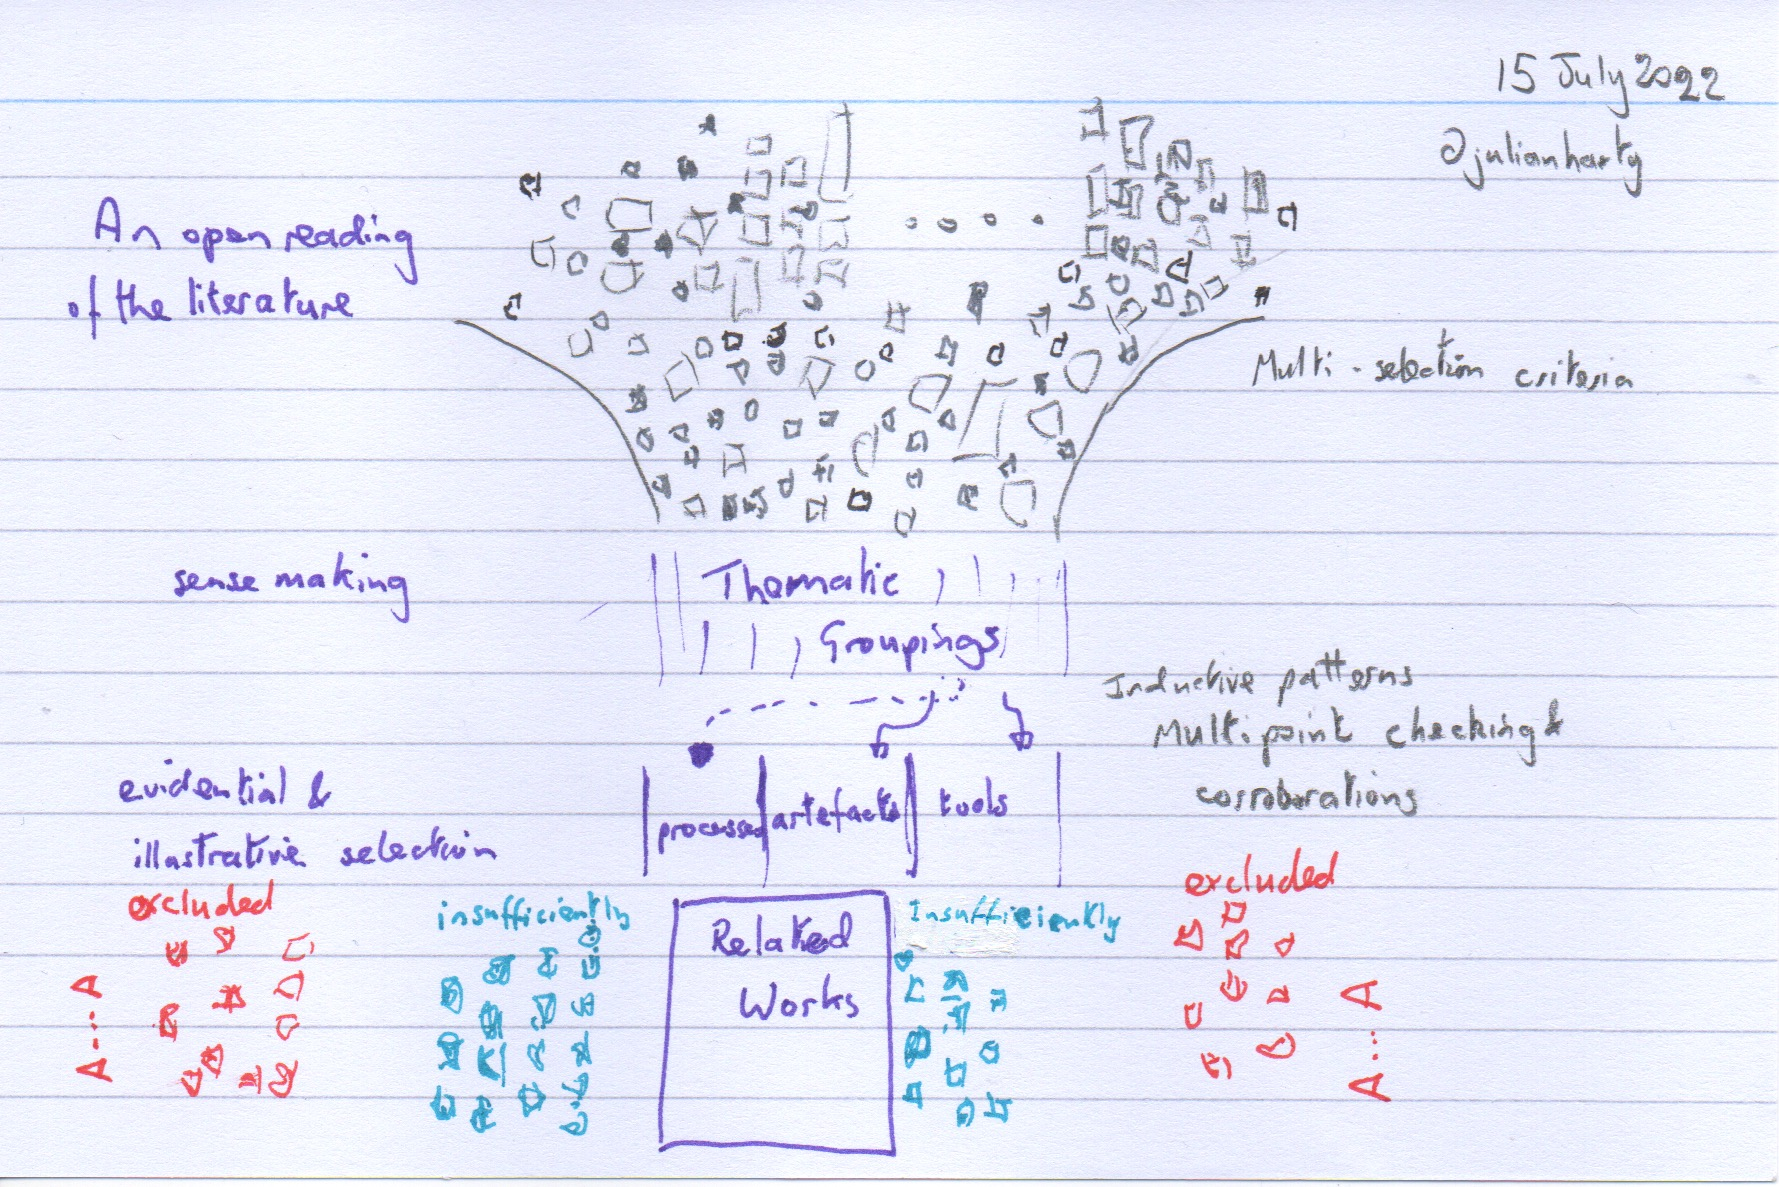
\includegraphics[width=\textwidth]{images/rough-sketches/literature-review-overview.jpeg}
    \caption{Overview of the literature review process and outcomes}
    \label{fig:literature-review-overview}
\end{figure}

Figure \ref{fig:literature-review-overview} illustrates my approach to researching prior work in the use of mobile analytics by app developers in order to measure and improve the stability/reliability of their mobile apps in the field/in the wild. Various searches, including keyword, tags, and related items, were incorporated into the searches. Initial sources included Google Scholar to find the more research oriented materials and Google Search particularly for grey materials, helped provide initial material to seed further searches. Specialist search tools were used where sites provided them, for instance on stack exchange sites such as StackOverflow, GitHub.com, acm.org, ieee.org, and medium.com their respective search engines were used frequently. Where practical copies of material has been preserved privately and backed up using at least one commercial, paid-for, cloud file storage service.

Multi-selection criteria are used to select material that appears of interest, relevant, and plausible. Generally bibliographic entries were obtained and these where checked for accuracy and completeness. Grey material seldom has a bibliographic entry, these were created, generally by hand, and preserved.

Through a process of sense-making, cross-checking, and corroborations various thematic groupings emerged together with potential relationships between the thematic groups. On reflection three clearly distinct and vital aspects emerged in the related work - the development practices used by mobile app developers, the artefacts they create and maintain, and the mobile analytics tools the developers use. These were further refined into six perspectives, using a three-by-two matrix: the x-axis incorporates the three aspects of processes, artefacts, and mobile analytics tools; the y-axis focuses on the current \emph{what is}, and \emph{what might be} in terms of making improvements.\todo{Arosha suggested three pillars which sounds good.}

The research materials and the bibliographic entries are maintained online. The most relevant ones are included in this thesis, many more are maintained in an `outtakes' folder, for example as `fieldstones'~\sidecite{weinberg2006weinberg} or in an insufficiently-related-works chapter. There's also an `excluded biography' file which helps reduce unnecessary repetition or groundhog day like practices. In the figure (\ref{fig:literature-review-overview}) the two \texttt{A ... A}'s wraps around - excluded works and insufficiently related works are similar distanced to this related works chapter.

In reading the literature various \textit{false friends} emerged, papers that first appear relevant because of their titles and/or abstracts but turn out to be on very different topics. 
Knowing about the concept of false friends and having pragmatic strategies to deal with them is important to avoid misunderstandings or misleading application of their work, 
based on \cite[p. 1833]{chamizodominguez2002_false_friends_their_origins_and_semantics_in_some_languages}. 
\textcite{shaw1989_comparing_conceptual_structures__consensus_conflict_correspondence_and_contrast} uses the term 'conflict`, where, \emph{``experts use [the] same terminology for different concepts"}~\cite[p. 3]{shaw1989_comparing_conceptual_structures__consensus_conflict_correspondence_and_contrast} (and, indeed, using their terminology here there is a `correspondence' where experts use two terms to describe the same concept e.g. `false friends' and `conflict' both describe the same concept.). For this research my work was limited to recognising false friends and identifying some examples. 

\subsection{Assessment criteria [TBC]}~\label{rw-assessment-criteria-topic}
For the purposes of this research there are two key dimensions in much of the research: 1) how grounded the work is in the real-world, and 2) how applicable it is to the real-world of developing mobile apps. Figure \ref{fig:grounded-and-applicable-boxplots} is a sketch of the two dimensions with five example topics. We will cover these topics shortly, % TODO complete the forward links.
before we do there are several pertinent research topics for general software development that help provide context for developing mobile apps.

\begin{figure}
    \centering
    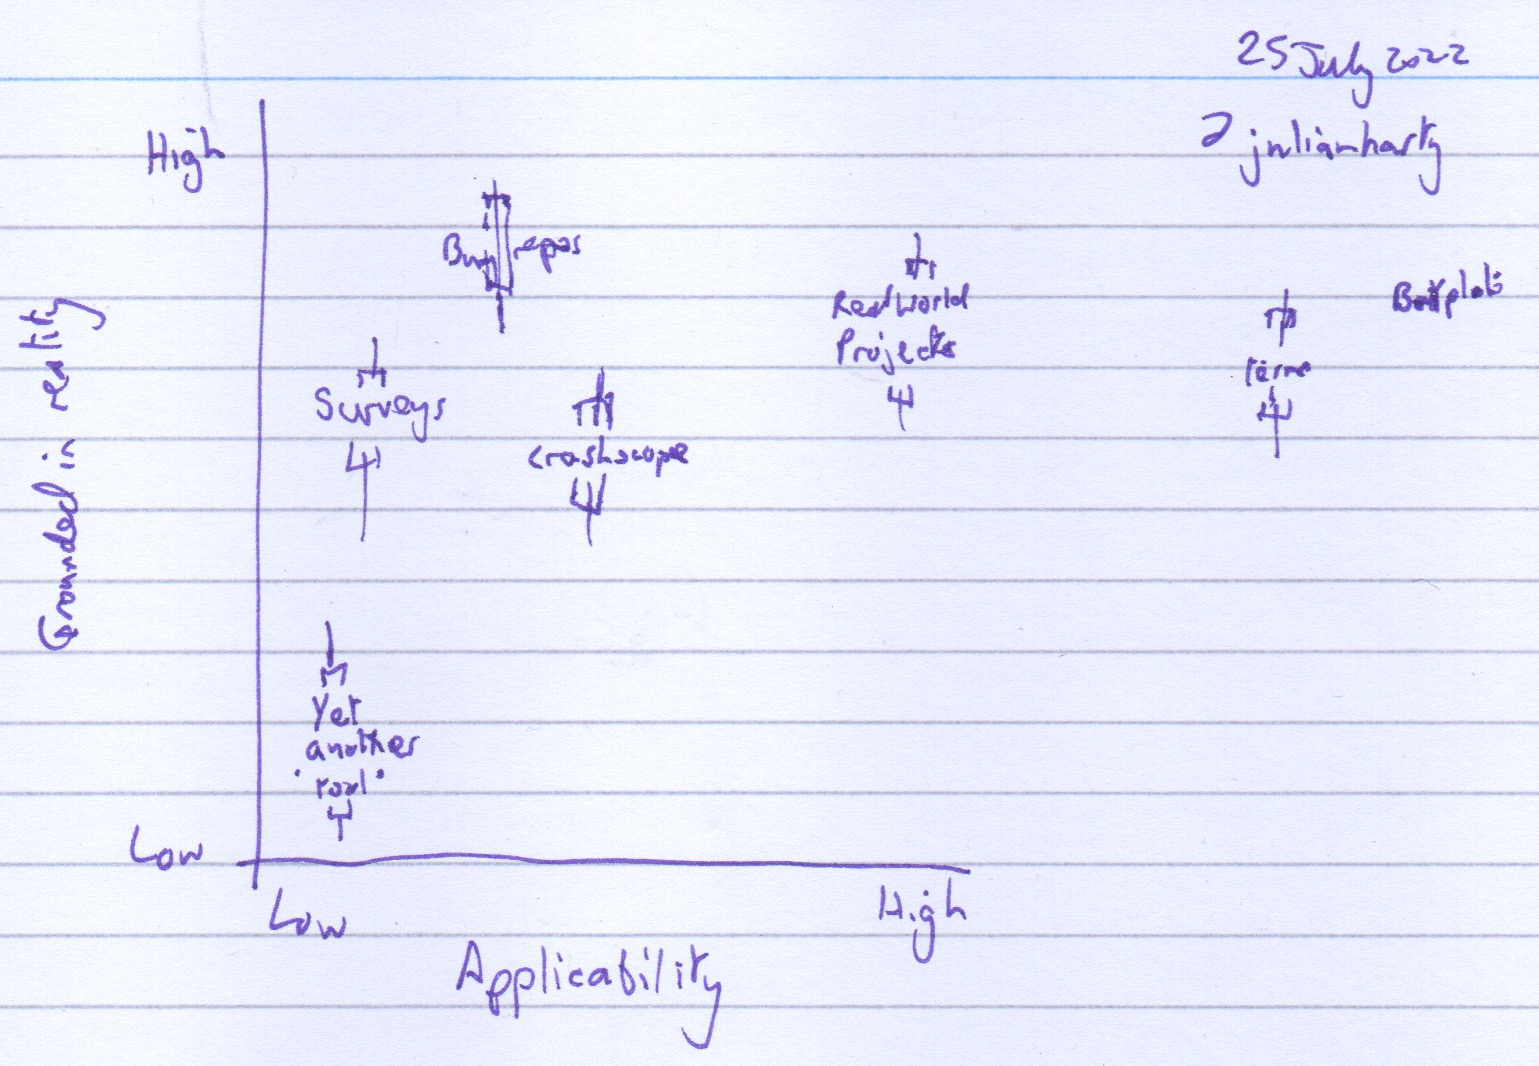
\includegraphics[width=\linewidth]{images/rough-sketches/grounded-and-applicable.jpeg}
    \caption{Box-plots visualising various research in mobile app software development}
    \label{fig:grounded-and-applicable-boxplots}
\end{figure}


So somehow I should aim to have the chapter structured with the following topics:\todo{This is a note to myself and needs replacing as I refine the chapter.}
\begin{enumerate}
    \item \textbf{Software Quality [Improvements] for mobile app developers}: Software Quality has been a contested topic for decades with no single accepted coherent agreement on what form(s) it takes, how software quality is measured, etc. Then comes the similarly vexed challenge of determining the concept and application of improvement in the quality/qualities of software. 
    \item \textbf{Mobile Analytics}: Research into \textbf{Processes, artefacts, and tools} necessary when using mobile analytics for improving software quality/qualities. These groupings emerged during the analysis of the literature and through understanding the practices of app developers.
    \begin{itemize}
        \item \textbf{Processes}: a.k.a. Analytics in Use - research into the processes developers use when they use mobile analytics
        \item \textbf{Artefacts}: things the developers create and maintain as part of their development work. Some of these are generated, in particular the app binary that is destined for end users once delivered by the app store.
        \item \textbf{Mobile Analytics Tools}: that the app developers use are worth researching in order to learn about their characteristics.
    \end{itemize}
\end{enumerate}

\subsection{Software Quality Improvements for mobile app developers}~\label{rw-software-quality-improvements-for-mobile-app-devs-topic}
Here topics might include the measures that have been used by app developers to measure software quality - as confirmed by research literature and grey materials. I suspect this is where I'd include sources of information about software quality (\secref{rw-sources-of-info-on-software-quality-for-devs-of-mobile-apps}).

\subsection{Development Processes for mobile apps}~\label{rw-devt-processes-for-mobile-apps}
Here topics include how the developers are perceived to work when they develop mobile apps, how they spend their time, how they structure and organise their work, etc. I suspect software testing fits here as well as how devs make mobile apps (the artefacts e.g. build scripts would go in the artefacts section).

\subsection{Artefacts for mobile apps}~\label{rw-artefacts-for-mobile-apps}
There's no end of research on artefacts from various subsets of opensource Android projects. Quite how well these reflect the population of shipping mobile apps (in Google Play in particular) is open to discussion. I can potentially include my joint research on logging practices as we aimed to only analyse projects where the codebase was actively maintained, etc. Research into logging practices by devs might also fit here (however how they use logging would be part of the section on development processes).

\subsection{Mobile Analytics (and Mobile Analytics tools)}~\label{rw-mobile-analytics-and-tools-topic}
I think it's germane to include research on the use of mobile analytics and any research into the tools, including the SDKs, data leakage, privacy, etc.

\subsection{Thoughts on the above organisation of the related works}~\label{rw-thoughts-on-organisation-of-the-rw}
As I've written the notes for each of the previous subsections I've had several instances where I've written about a single topic split across processes and artefacts. Perhaps it'd be better to keep the topics together and then summarise the topics by explaining there's a key distinction between the artefacts that exist and how they're used in practice. If so, then the alignment with the six perspectives would occur towards the end of this chapter rather than being used throughout. Let's see.

